\section{Результаты}

Все реализации были тестированы на корректность на аналитическом решении (свободной дифракции гауссова пучка),
и на консервативность.

Представлены результаты замеров времени работы алгоритма с использованием преобразования Фурье при различных комбинациях параметров, выбранных для анализа их влияния на время работы программы.
Запуск и замеры времени осуществлялись на кластере СКИФ МГУ <<Чебышёв>>.

    \begin{figure}[h!]
        \begin{center}
            \begin{minipage}{0.45\linewidth}
                \center{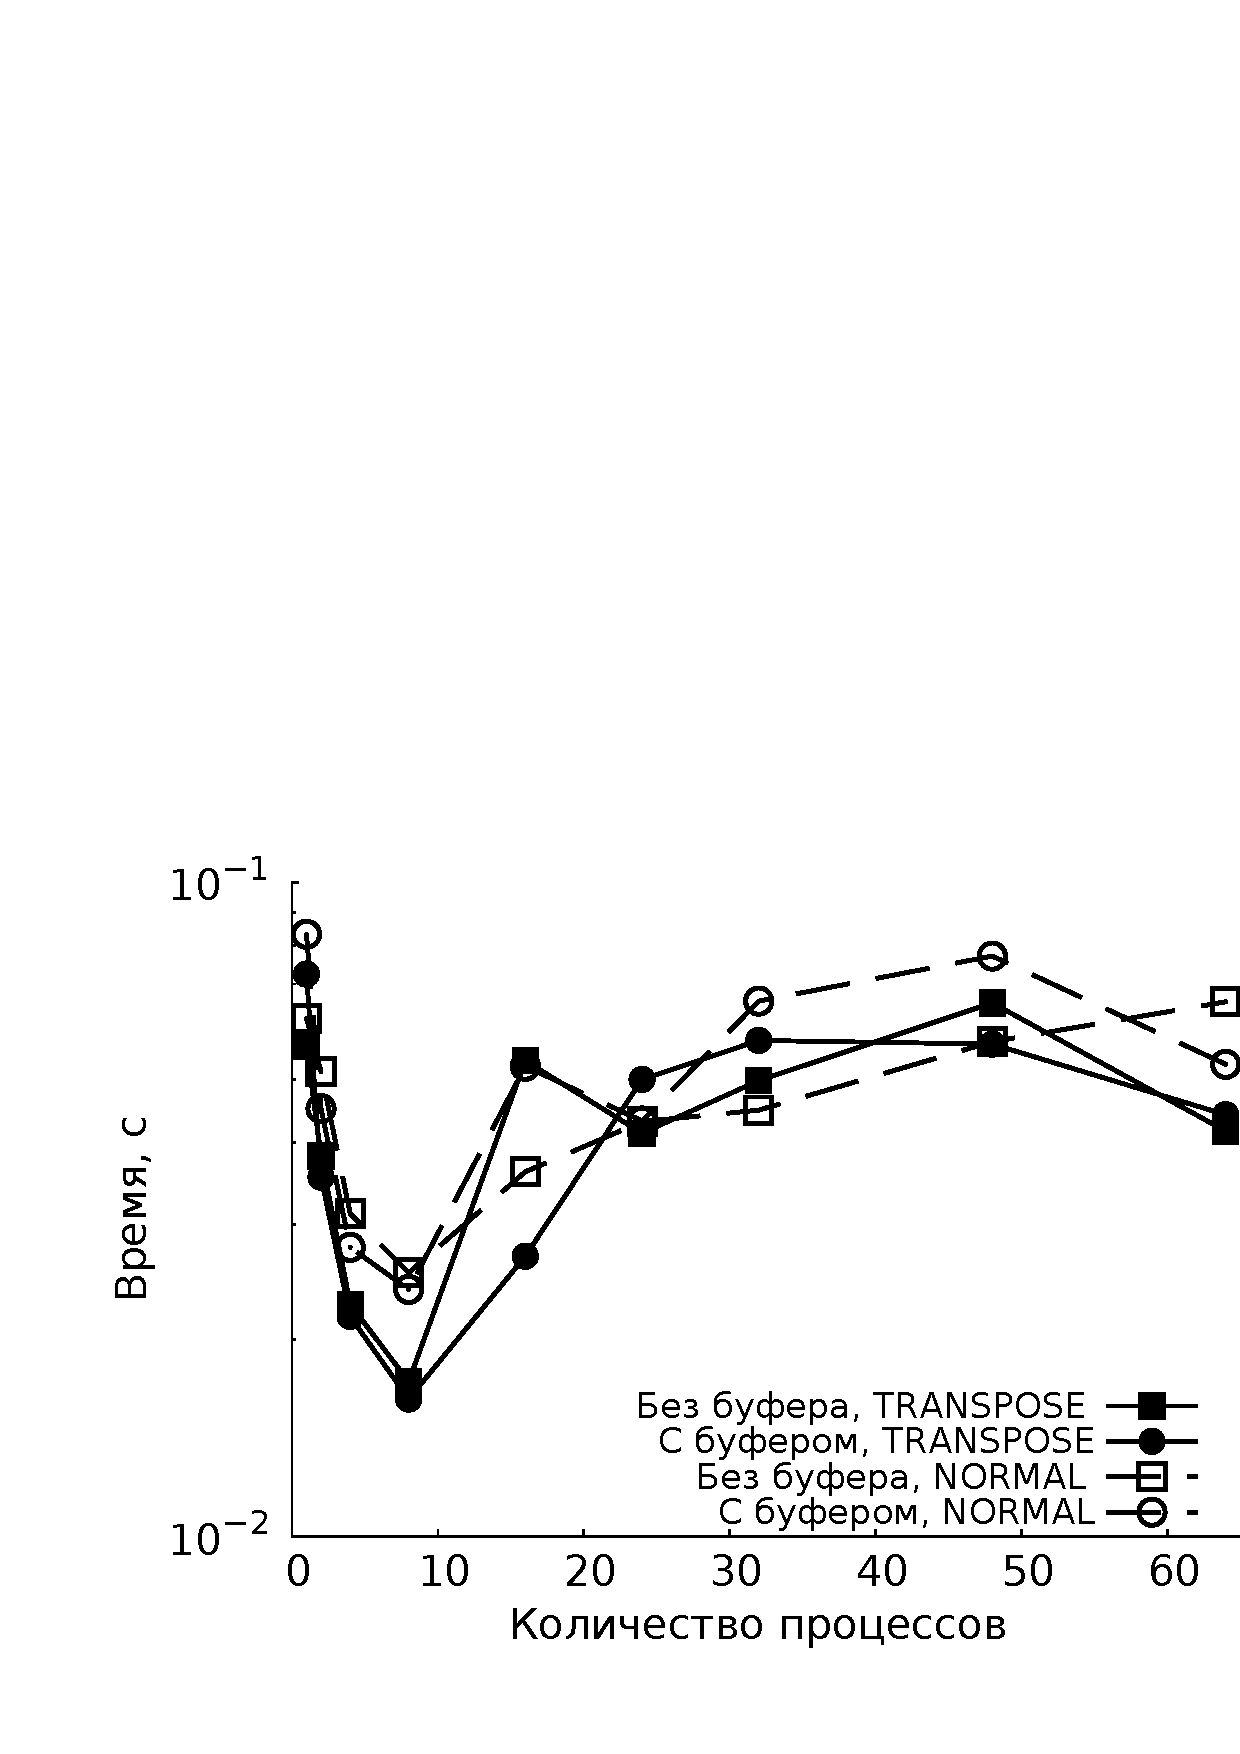
\includegraphics[width=0.95\linewidth]{\graphsdir/Skif/FFTW_compare_N512_nomeasure_all.png}}
                \caption{Время работы Фурье-алгоритма в зависимости от количества процессов. Размер матрицы 512. Флаг FFTW\_ESTIMATE.}
                \label{gr:Fourier512Nomeasure}
            \end{minipage}
            \hfill
            \begin{minipage}{0.45\linewidth}
                \center{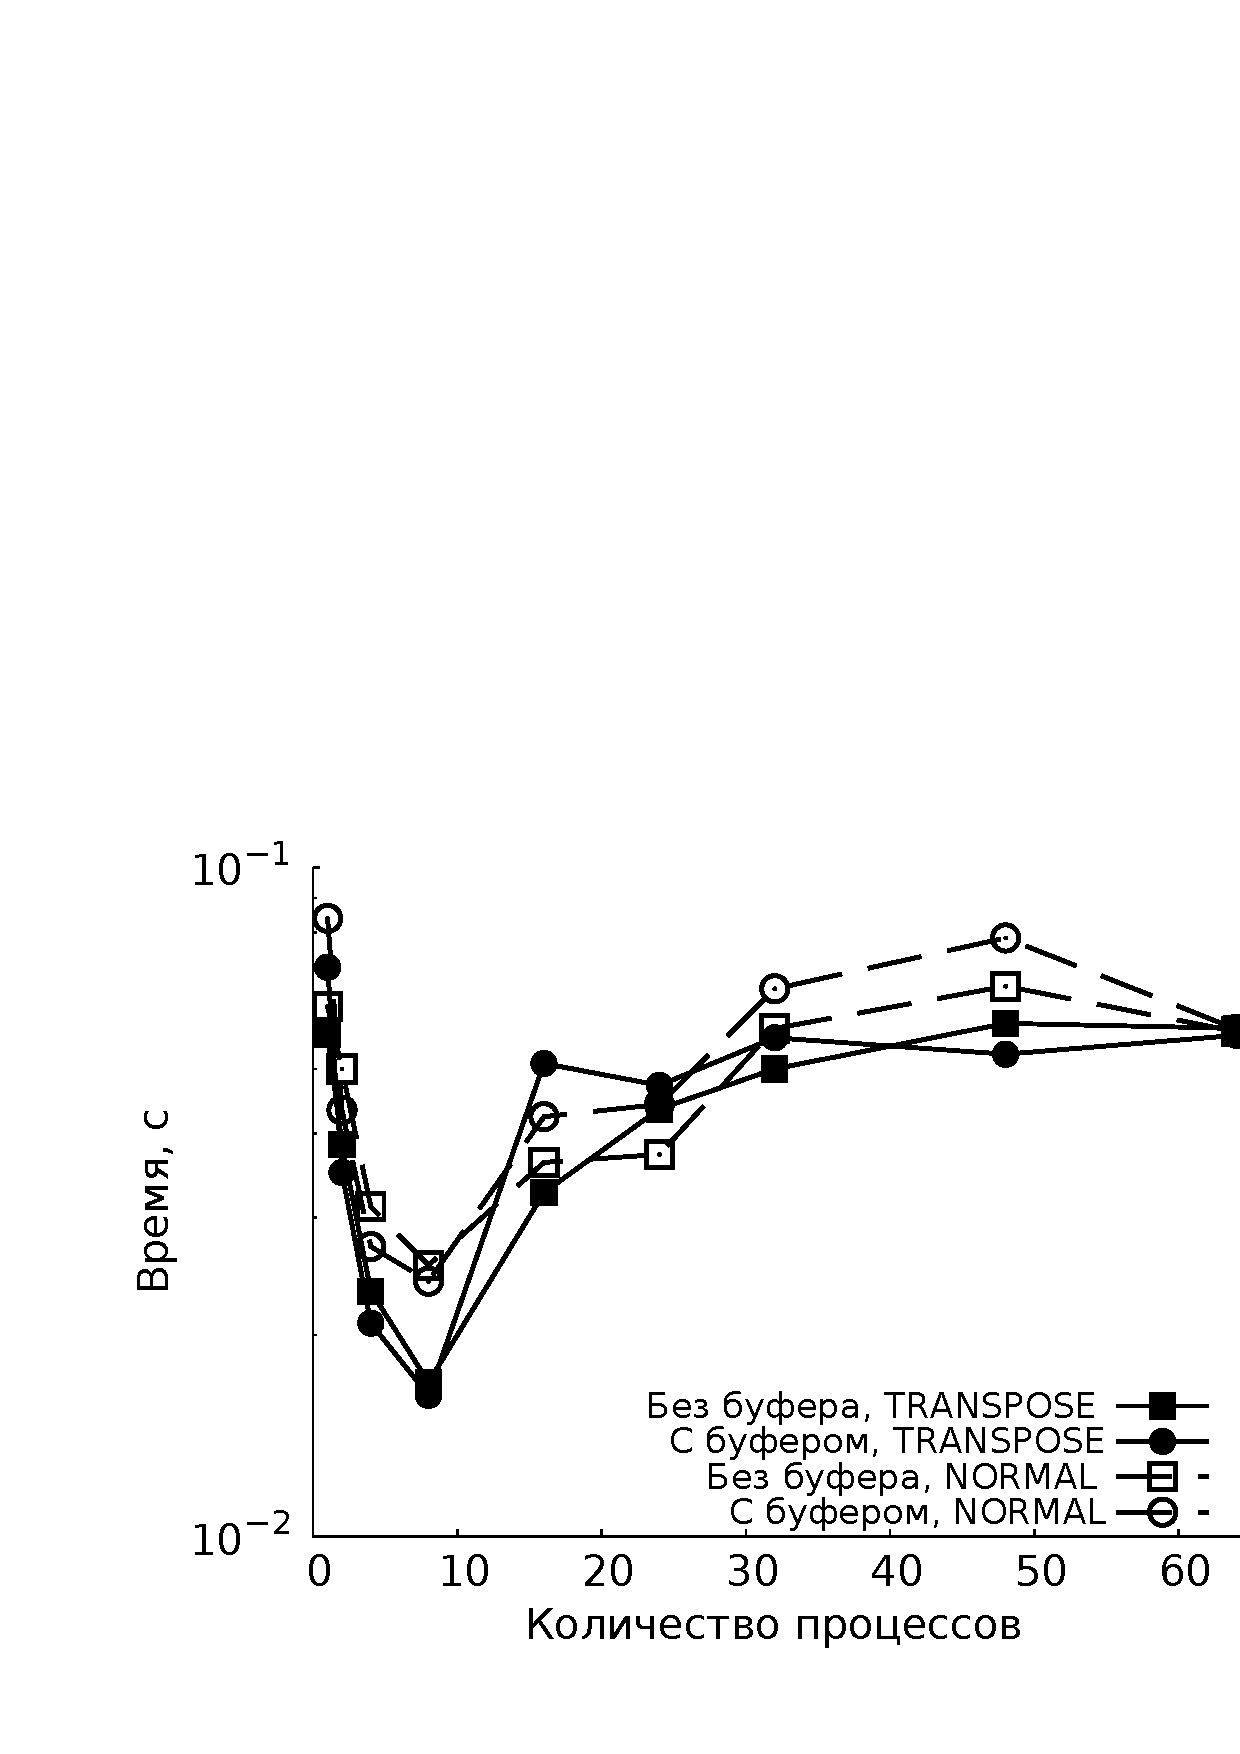
\includegraphics[width=0.95\linewidth]{\graphsdir/Skif/FFTW_compare_N512_measure_all.png}}
                \caption{Время работы Фурье-алгоритма в зависимости от количества процессов. Размер матрицы 512. Флаг FFTW\_MEASURE.}
                \label{gr:Fourier512Measure}
            \end{minipage}
        \end{center}
    \end{figure}

Из представленных на рис. \ref{gr:Fourier512Nomeasure}, \ref{gr:Fourier512Measure} графиков видно, что использование более 16 процессоров является неэффективным для размера матрицы $N = 512$, так как время работы программы возрастает по сравнению с временем работы программы при тех же параметрах на 8 процессорах.

	\begin{figure}[h!]
		\begin{center}
    		\begin{minipage}{0.48\linewidth}
				\center{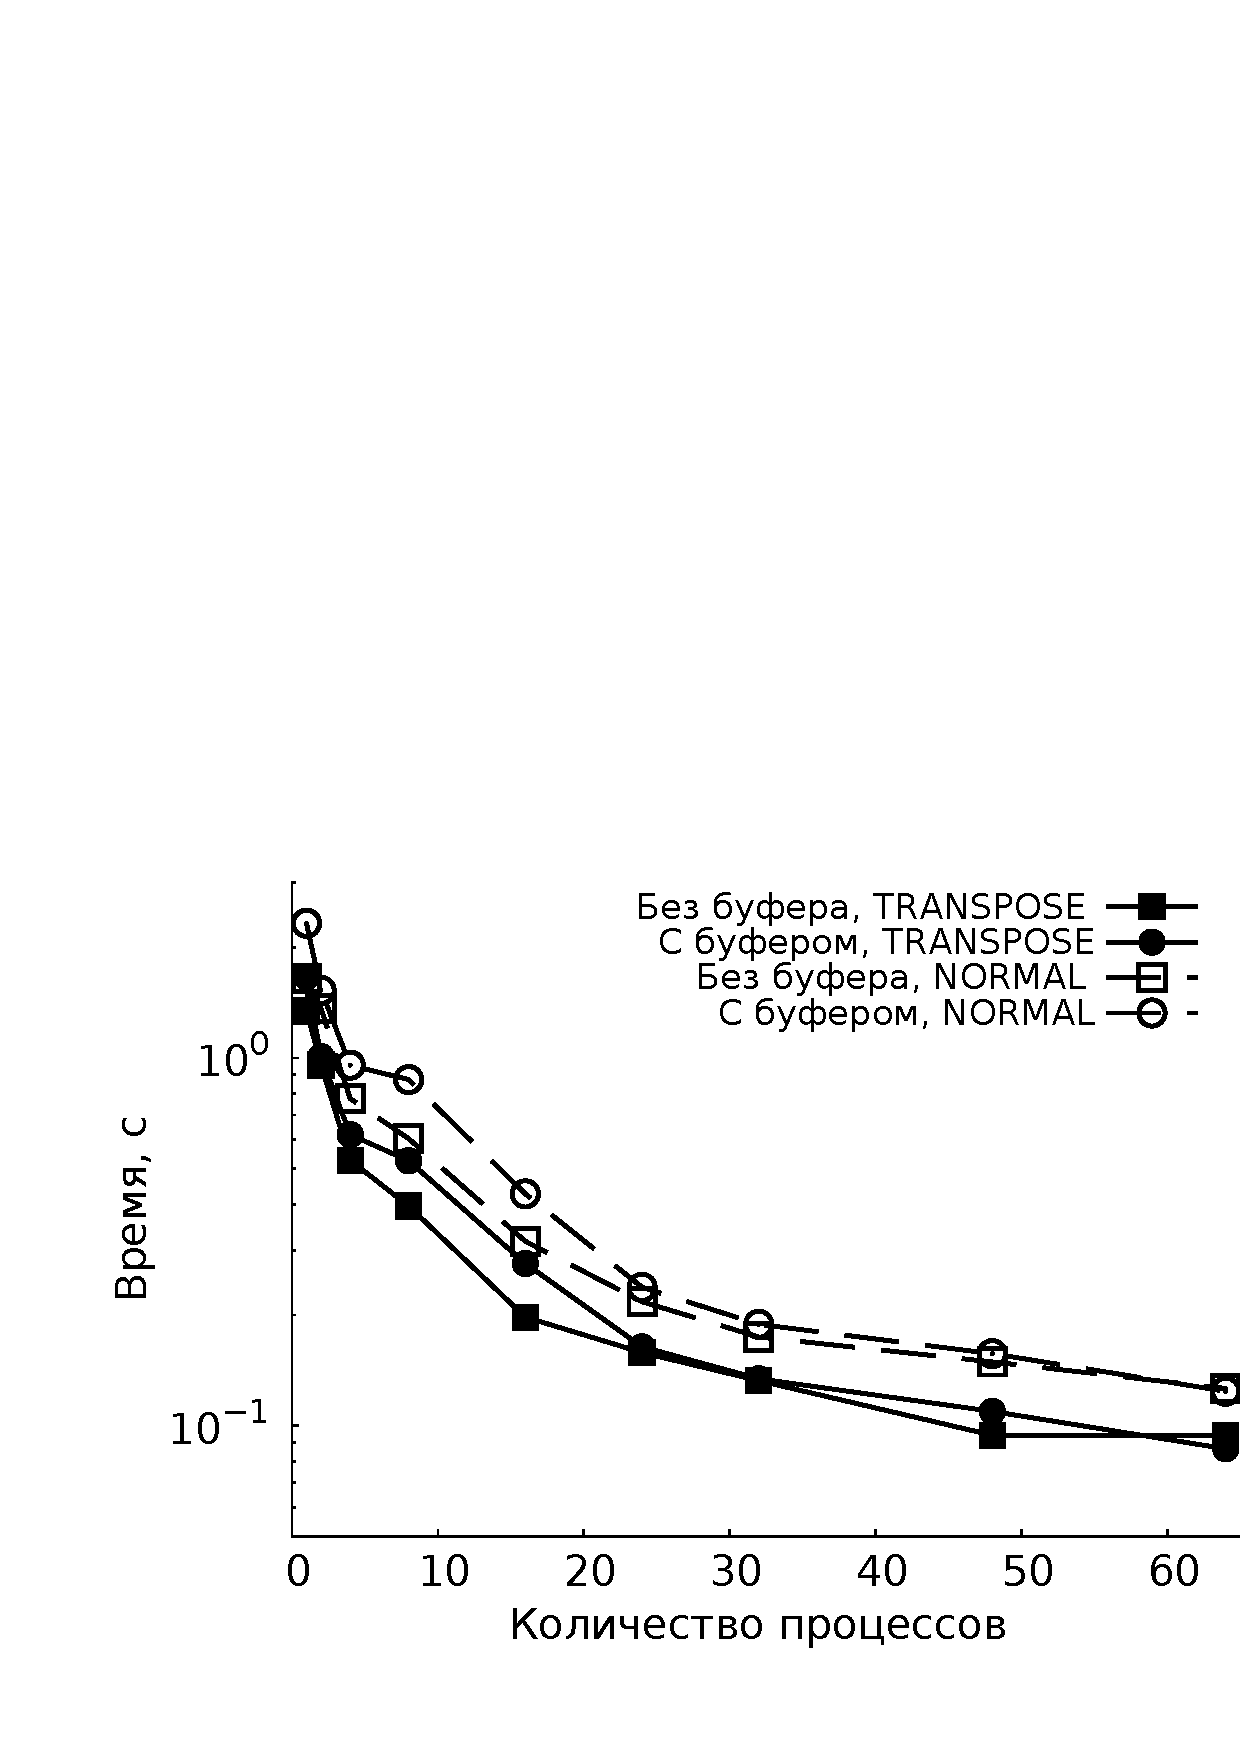
\includegraphics[width=0.95\linewidth]{\graphsdir/Skif/FFTW_compare_N2048_nomeasure_all.png}}
                \caption{Время работы Фурье-алгоритма в зависимости от количества процессов. Размер матрицы 2048. Флаг FFTW\_ESTIMATE.}
                \label{gr:Fourier2048Nomeasure}
			\end{minipage}
			\hfill
			\begin{minipage}{0.48\linewidth}
				\center{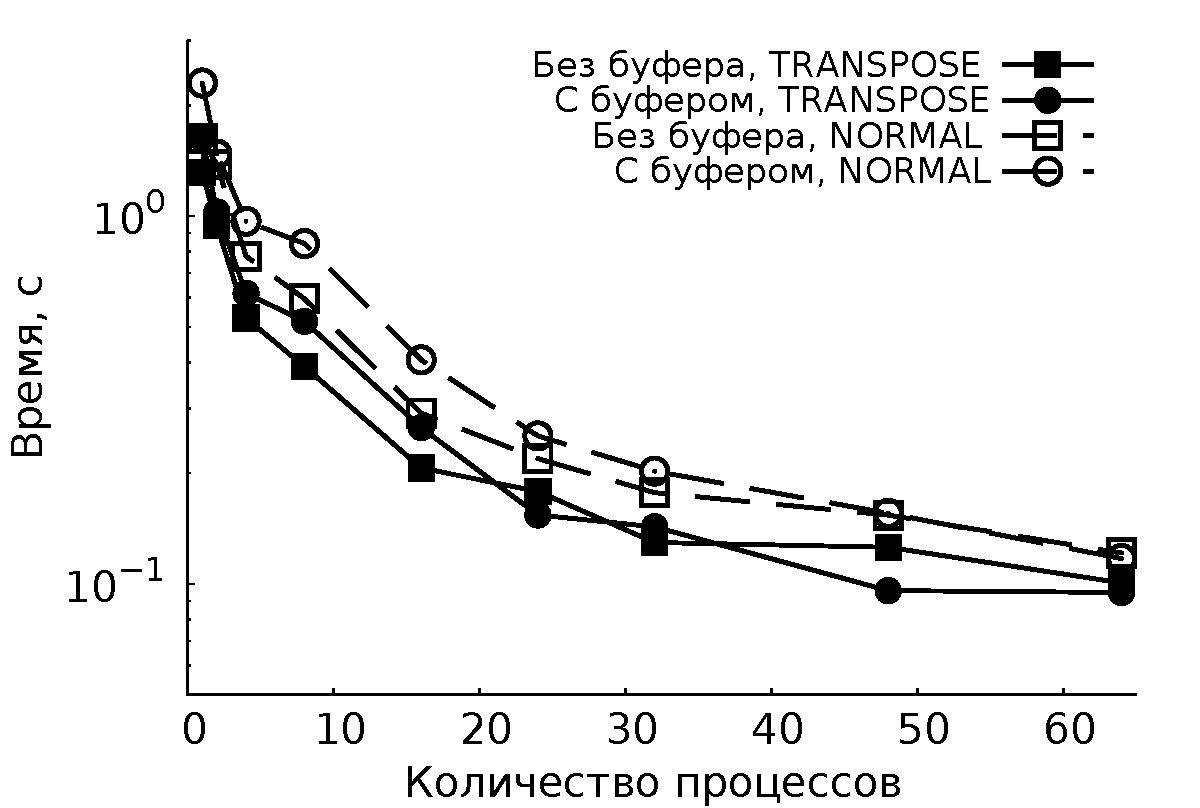
\includegraphics[width=0.95\linewidth]{\graphsdir/Skif/FFTW_compare_N2048_measure_all.png}}
                \caption{Время работы Фурье-алгоритма в зависимости от количества процессов. Размер матрицы 2048. Флаг FFTW\_MEASURE.}
                \label{gr:Fourier2048Measure}
			\end{minipage}
		\end{center}
	\end{figure}

Для размера матрицы 2048, как видно из рис. \ref{gr:Fourier2048Nomeasure}, \ref{gr:Fourier2048Measure} увеличение числа процессоров от 1 до 16 дает ощутимое уменьшение времени работы программы.
		
	\begin{figure}[h!]
		\begin{center}
			\begin{minipage}{0.45\linewidth}
        		\center{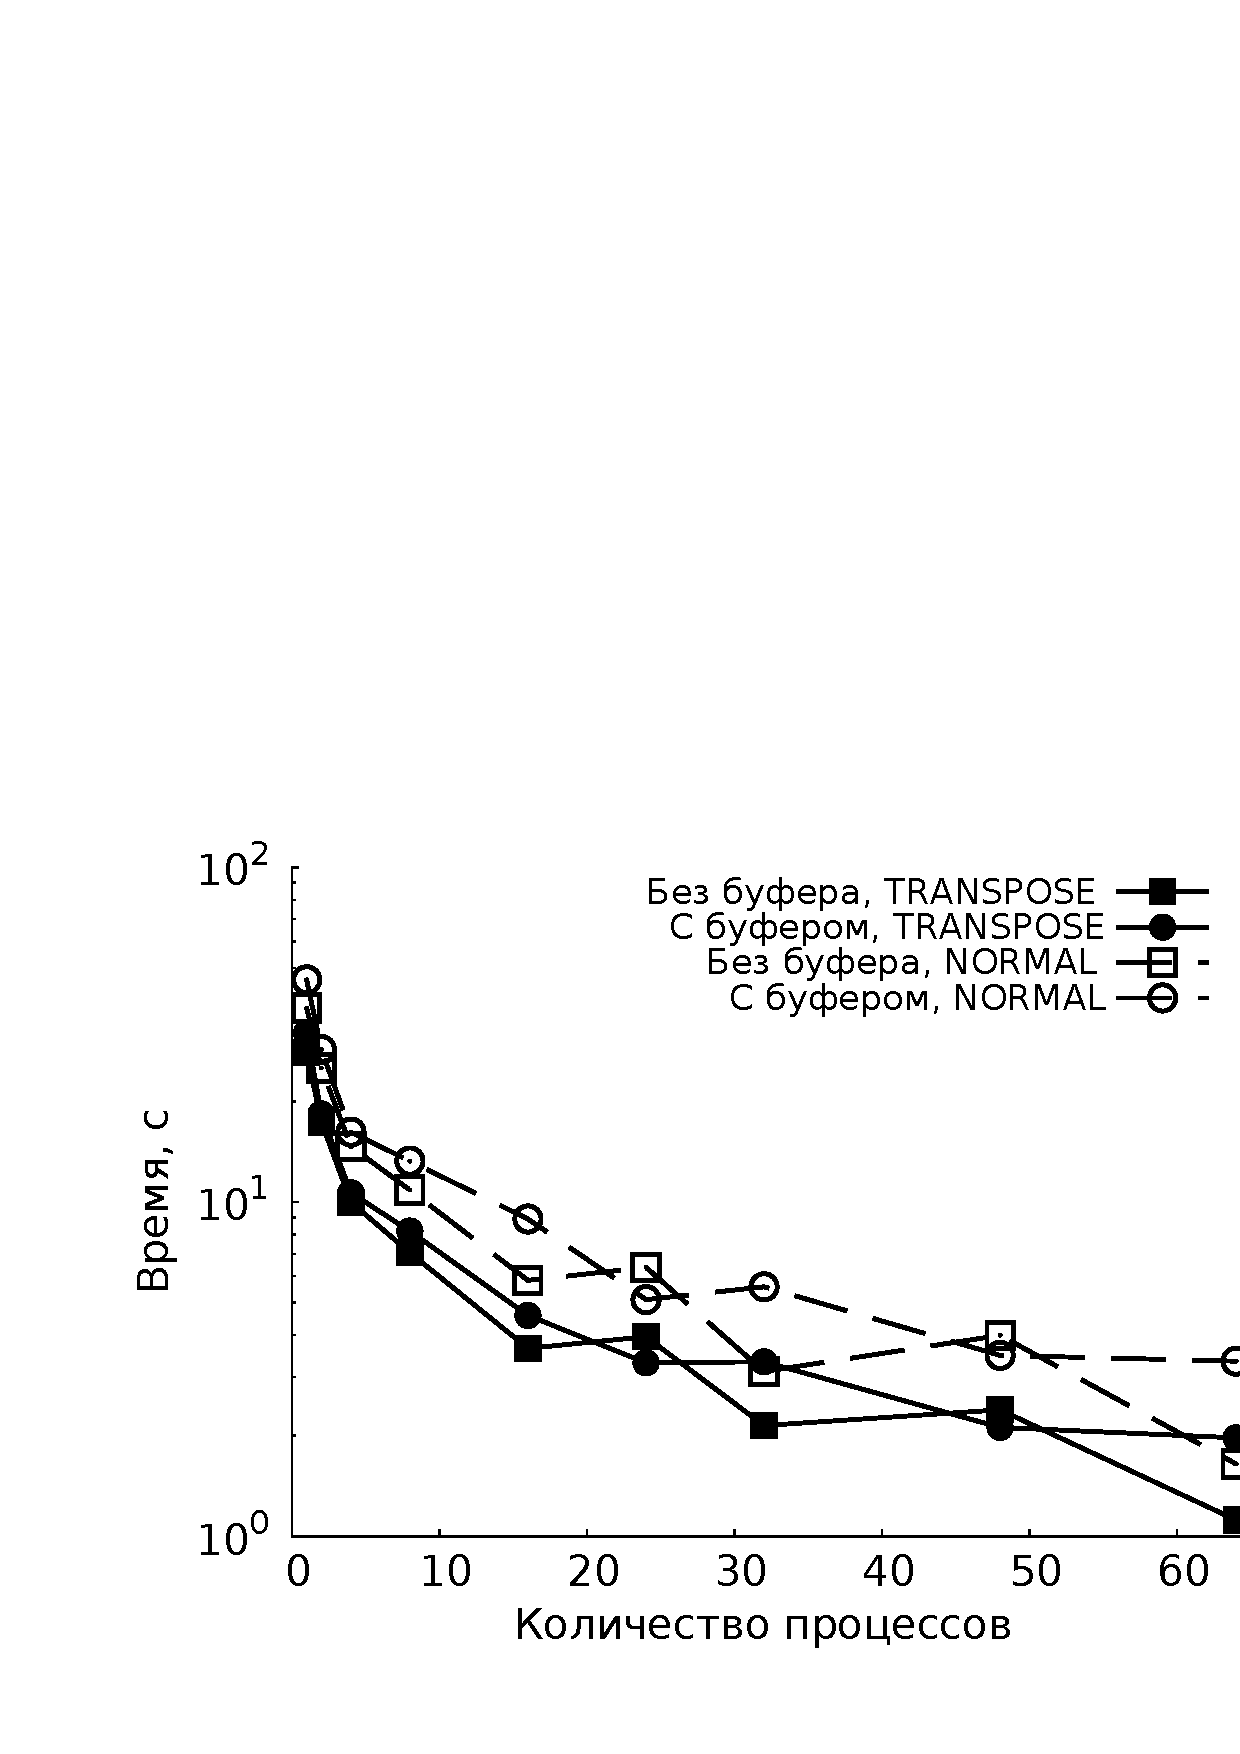
\includegraphics[width=0.95\linewidth]{\graphsdir/Skif/FFTW_compare_N8192_nomeasure_all.png}}
                \caption{Время работы Фурье-алгоритма в зависимости от количества процессов. Размер матрицы 8192. Флаг FFTW\_ESTIMATE.}
                \label{gr:Fourier8192Nomeasure}
			\end{minipage}
			\hfill
			\begin{minipage}{0.45\linewidth}
				\center{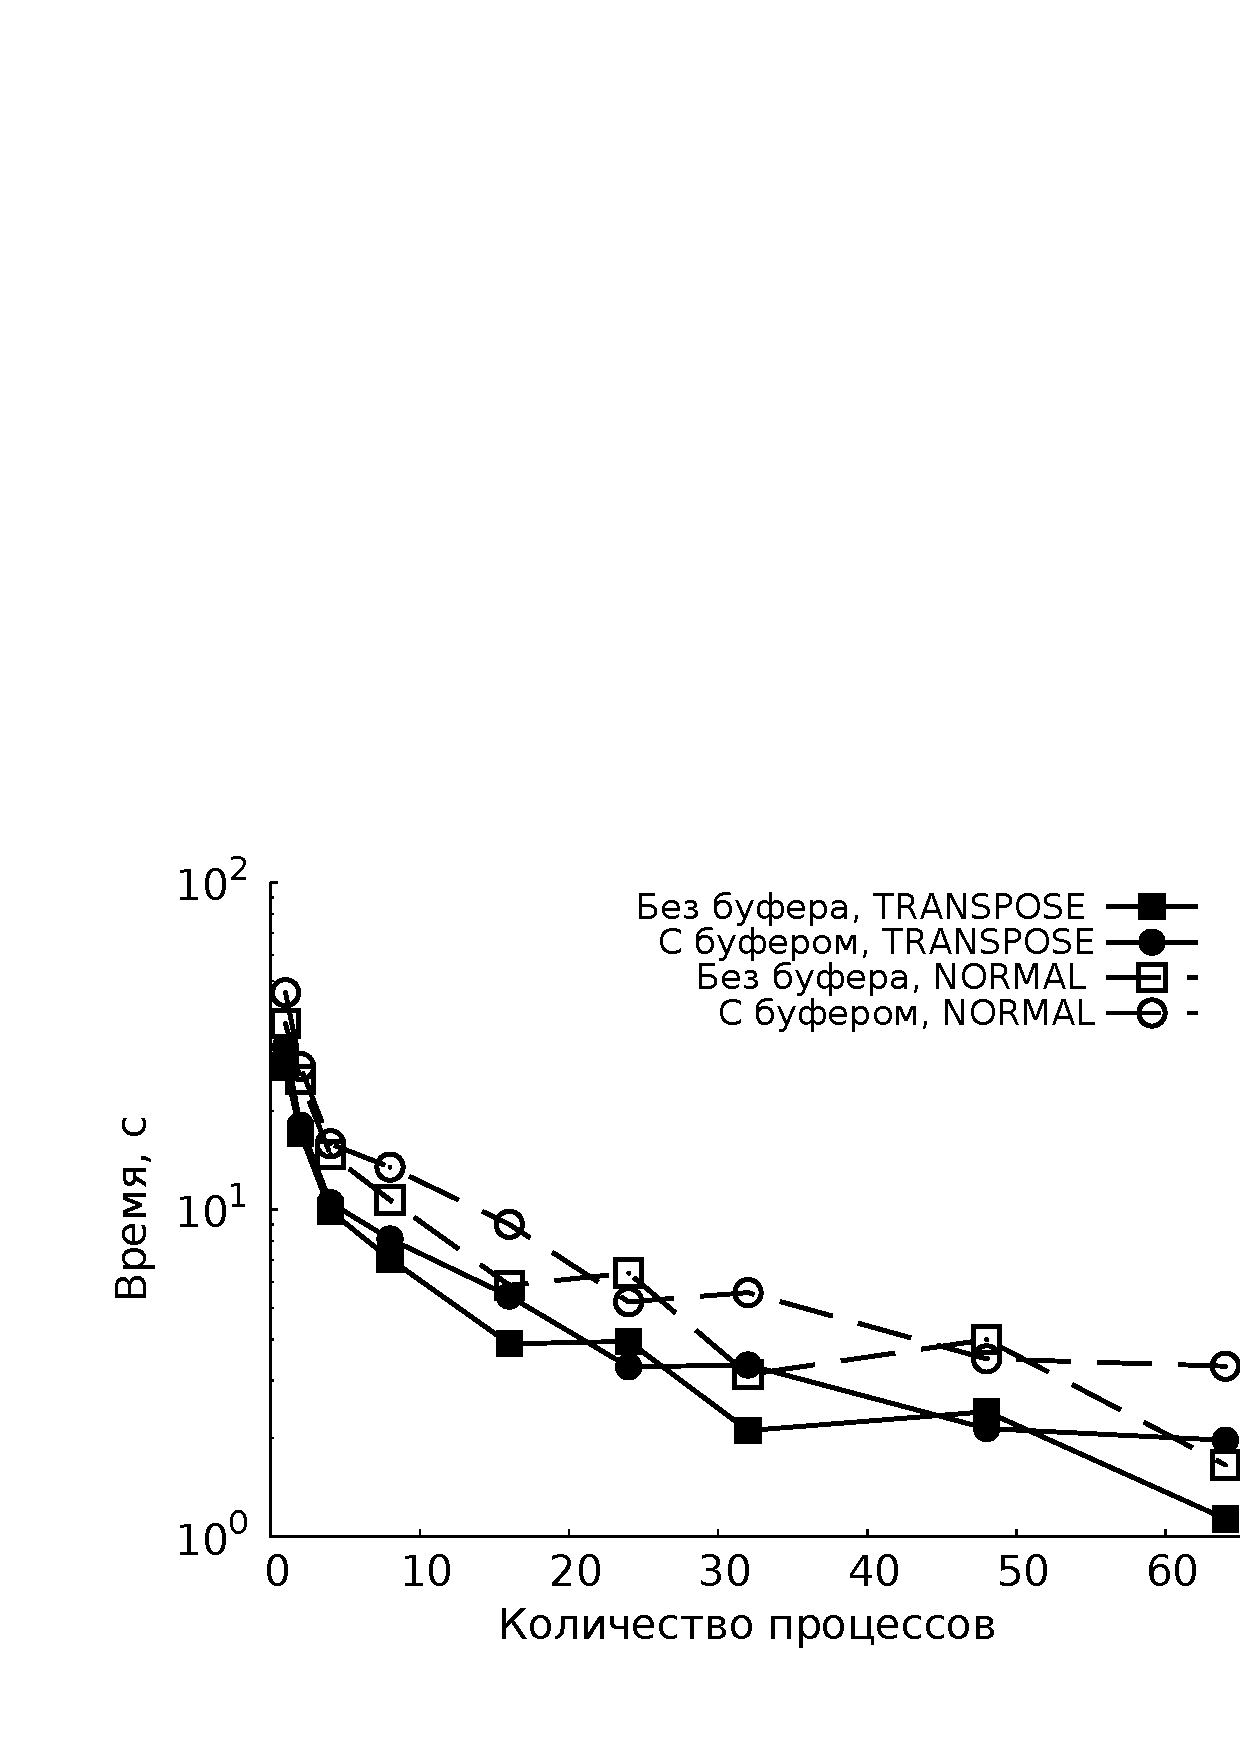
\includegraphics[width=0.95\linewidth]{\graphsdir/Skif/FFTW_compare_N8192_measure_all.png}}
                \caption{Время работы Фурье-алгоритма в зависимости от количества процессов. Размер матрицы 8192. Флаг FFTW\_MEASURE.}
                \label{gr:Fourier8192Measure}
			\end{minipage}
		\end{center}
	\end{figure}

При использовании матрицы размером 8192 времена работы программы увеличиваются соответственно, что позволяет увидеть более четко различие во временах работы программы при использовании различных комбинаций флагов.

Из графиков на рис. \ref{gr:Fourier512Nomeasure}--\ref{gr:Fourier8192Measure} видно, что использования флага FFTW\_MEASURE не приводит к убыстрению работы алгоритма, что связано прежде всего с малым количеством расчетных узлов.
Кроме того, использование буфера не только не привело к ускорению алгоритма, но, наоборот, несколько затормозило его.
По представленным результатам был сделан вывод, что лучшее враг хорошего. Скорость работы алгоритма с ключом FFTW\_TRANSPOSED\_ORDER, как и ожидалось, оказалась выше, чем с ключом FFTW\_NORMAL\_ORDER.

Было проведено исследование зависимости времени работы алгоритма от используемых ключей компиляции. Результаты представлены в табл. \ref{tab:compilers}.
    \begin{table}[ht]
        \centering
        \begin{tabular}{ | c | c | c | }
            \hline
            Опция		&	$np=8$	&	$np=16$ \\
            \hline
            -O2	(по умолчанию)	&	9.0 с		&	5.0 с \\
            \hline
            -О1		&	9.2 с	 	&	5.3 с \\
            \hline
            -О3		&	8.8 с		&	5.1 с \\
            \hline
            -Оs		&	9.0 с		&	5.2 с \\
            \hline
            -fast	&	8.9 с		&	5.2 с \\
            \hline
        \end{tabular}
        \begin{center}
            \caption{Зависимость времени такта от опций компиляции.}\label{tab:compilers}
        \end{center}
    \end{table}

Таким образом, использование ключей компиляции не дало ощутимого уменьшения времени работы программы.

	\begin{figure}[h!]
		\begin{center}
			\begin{minipage}{0.45\linewidth}
				\center{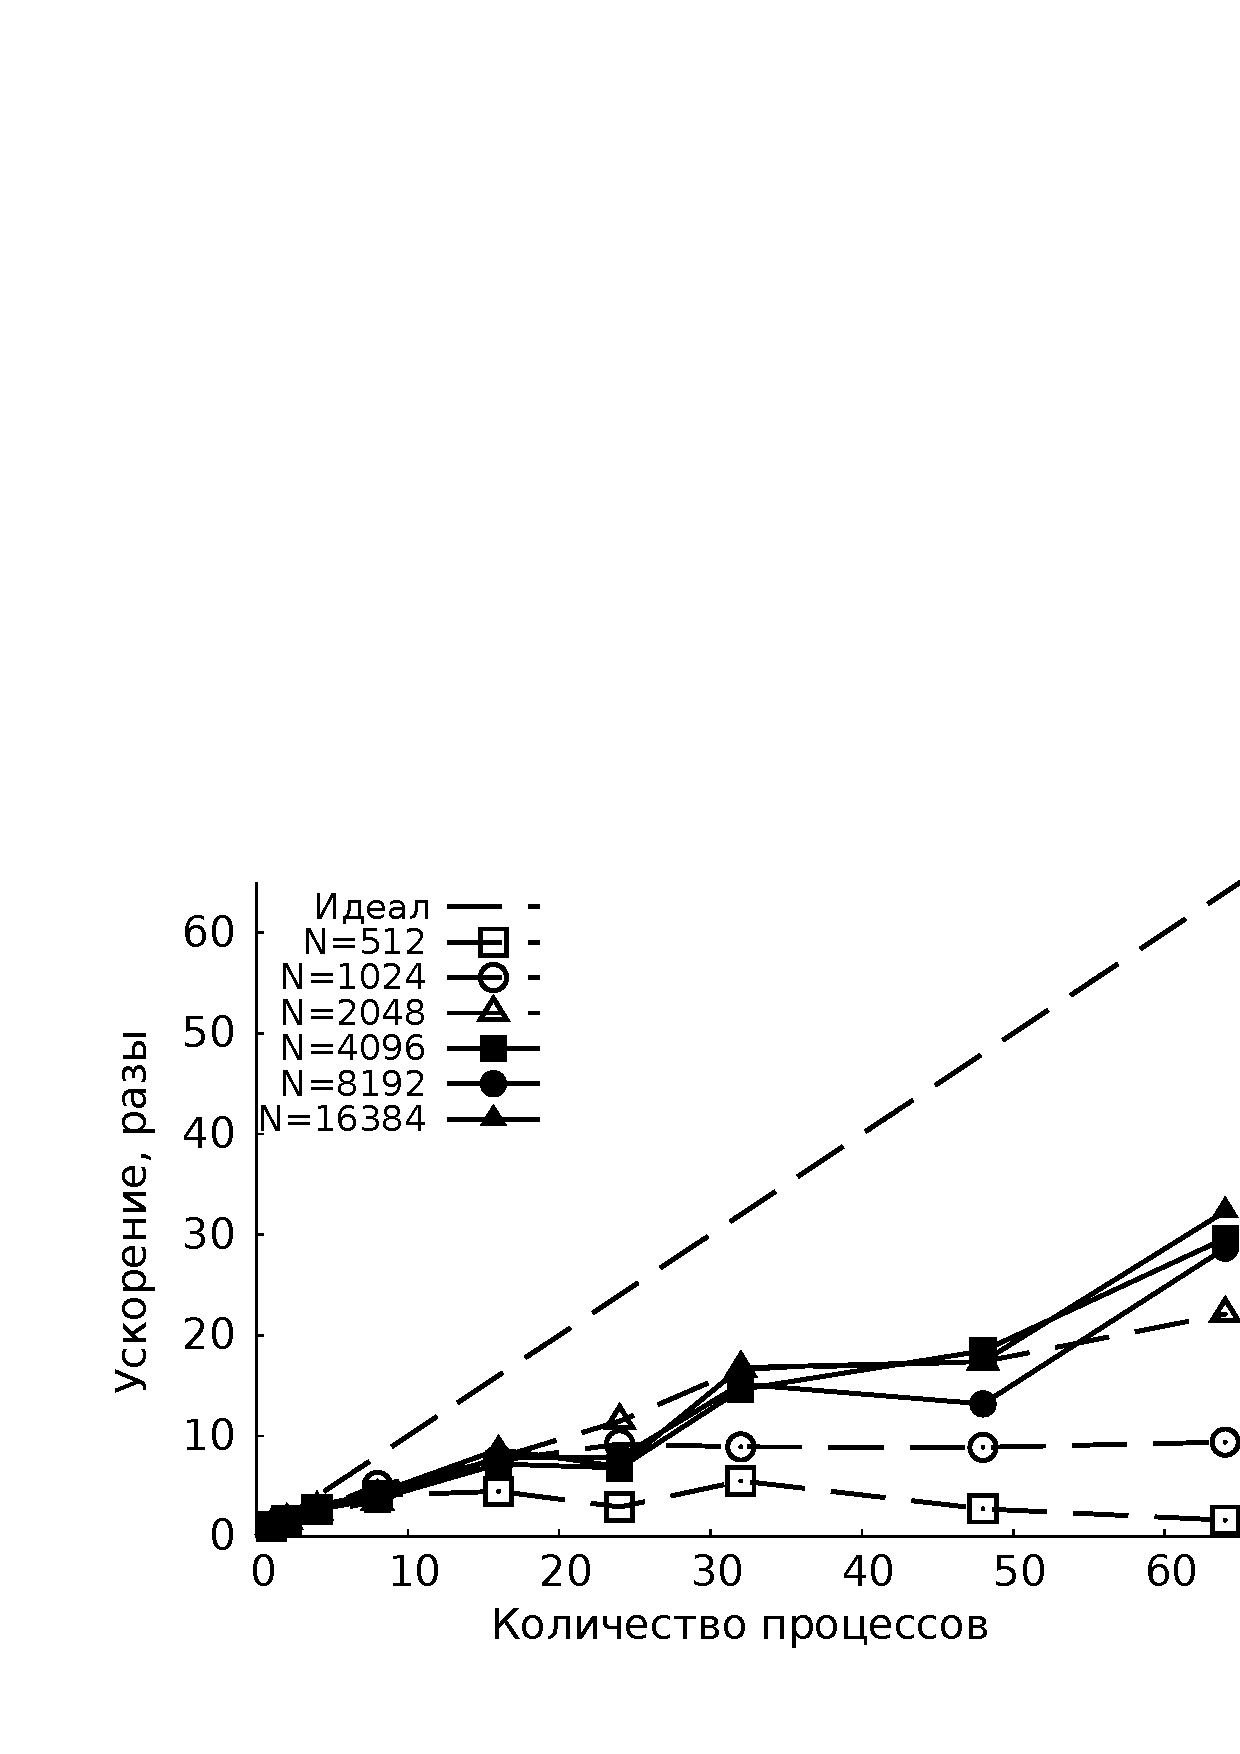
\includegraphics[width=0.95\linewidth]{\graphsdir/Skif/FFTW_acceleration_nosave_all.png}} \\
                \caption{Ускорение Фурье-алгоритма в зависимости от количества процессов для разных размеров матриц. Сохранение данных в файл не производилось.}
                \label{gr:SpeedupFourierNosave}
			\end{minipage}
			\hfill
			\begin{minipage}{0.45\linewidth}
				\center{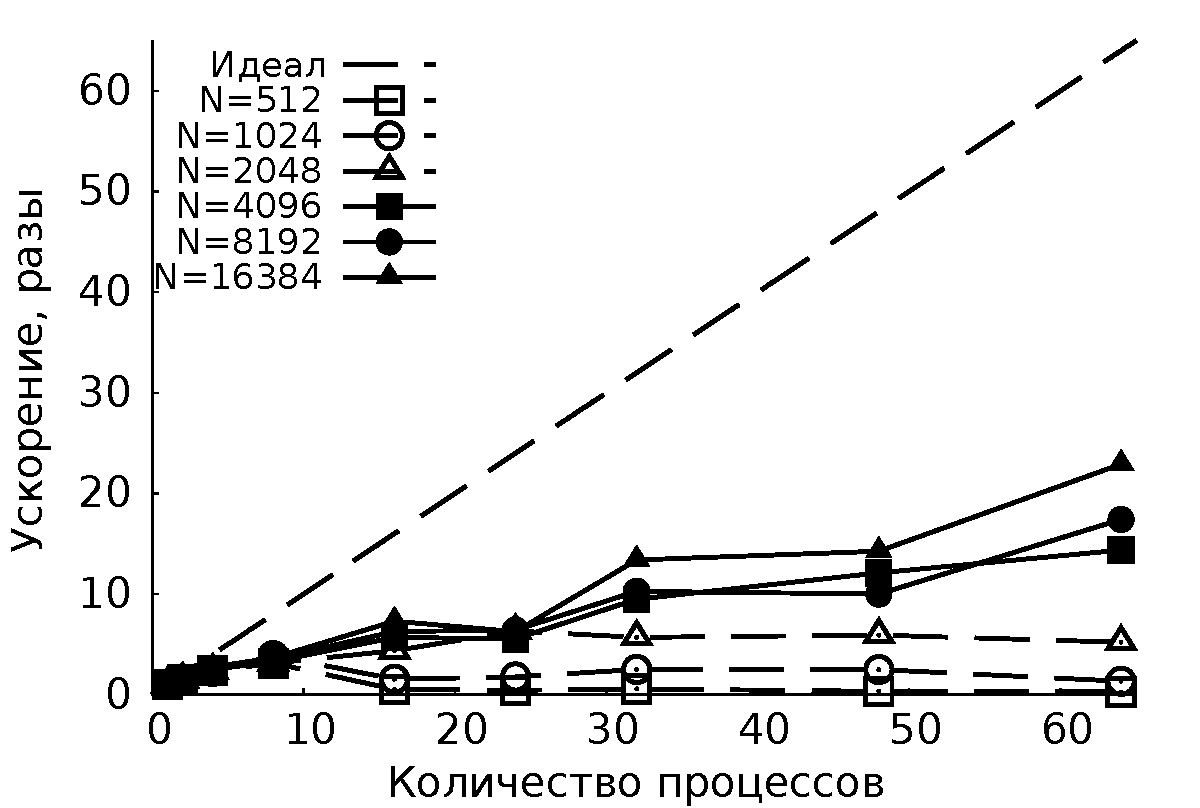
\includegraphics[width=0.95\linewidth]{\graphsdir/Skif/FFTW_acceleration_withsave_all.png}} \\
                \caption{Ускорение Фурье-алгоритма в зависимости от количества процессов для разных размеров матриц. Сохранение данных в файл производилось на каждом десятом шаге.}
                \label{gr:SpeedupFourierSave}
			\end{minipage}
		\end{center}
	\end{figure}

	\begin{figure}[h!]
		\begin{center}
			\begin{minipage}{0.45\linewidth}
				\center{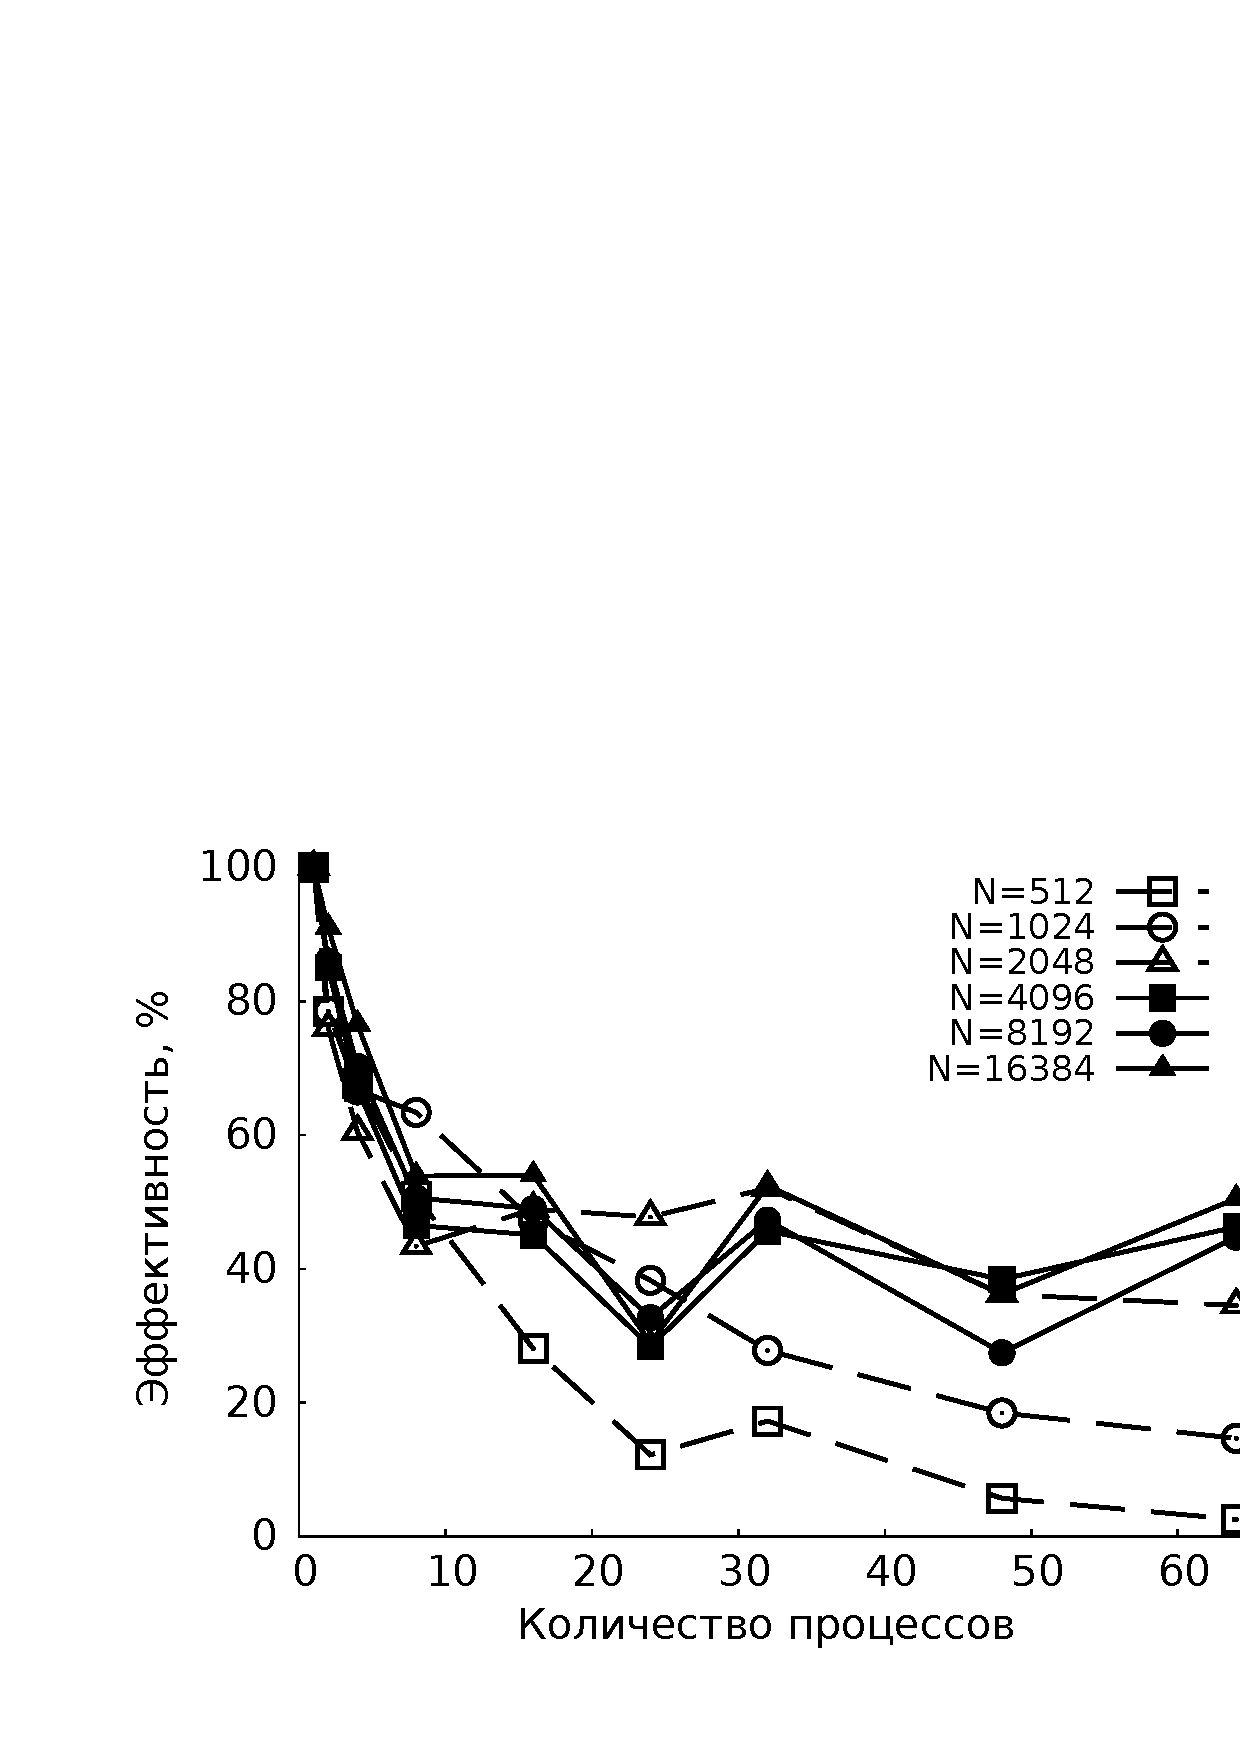
\includegraphics[width=0.95\linewidth]{\graphsdir/Skif/FFTW_efficiency_nosave_all.png}} \\
                \caption{Эффективность Фурье-алгоритма в зависимости от количества процессов для разных размеров матриц. Сохранение данных в файл не производилось.}
                \label{gr:EfficiencyFourierNosave}
			\end{minipage}
			\hfill
			\begin{minipage}{0.45\linewidth}
				\center{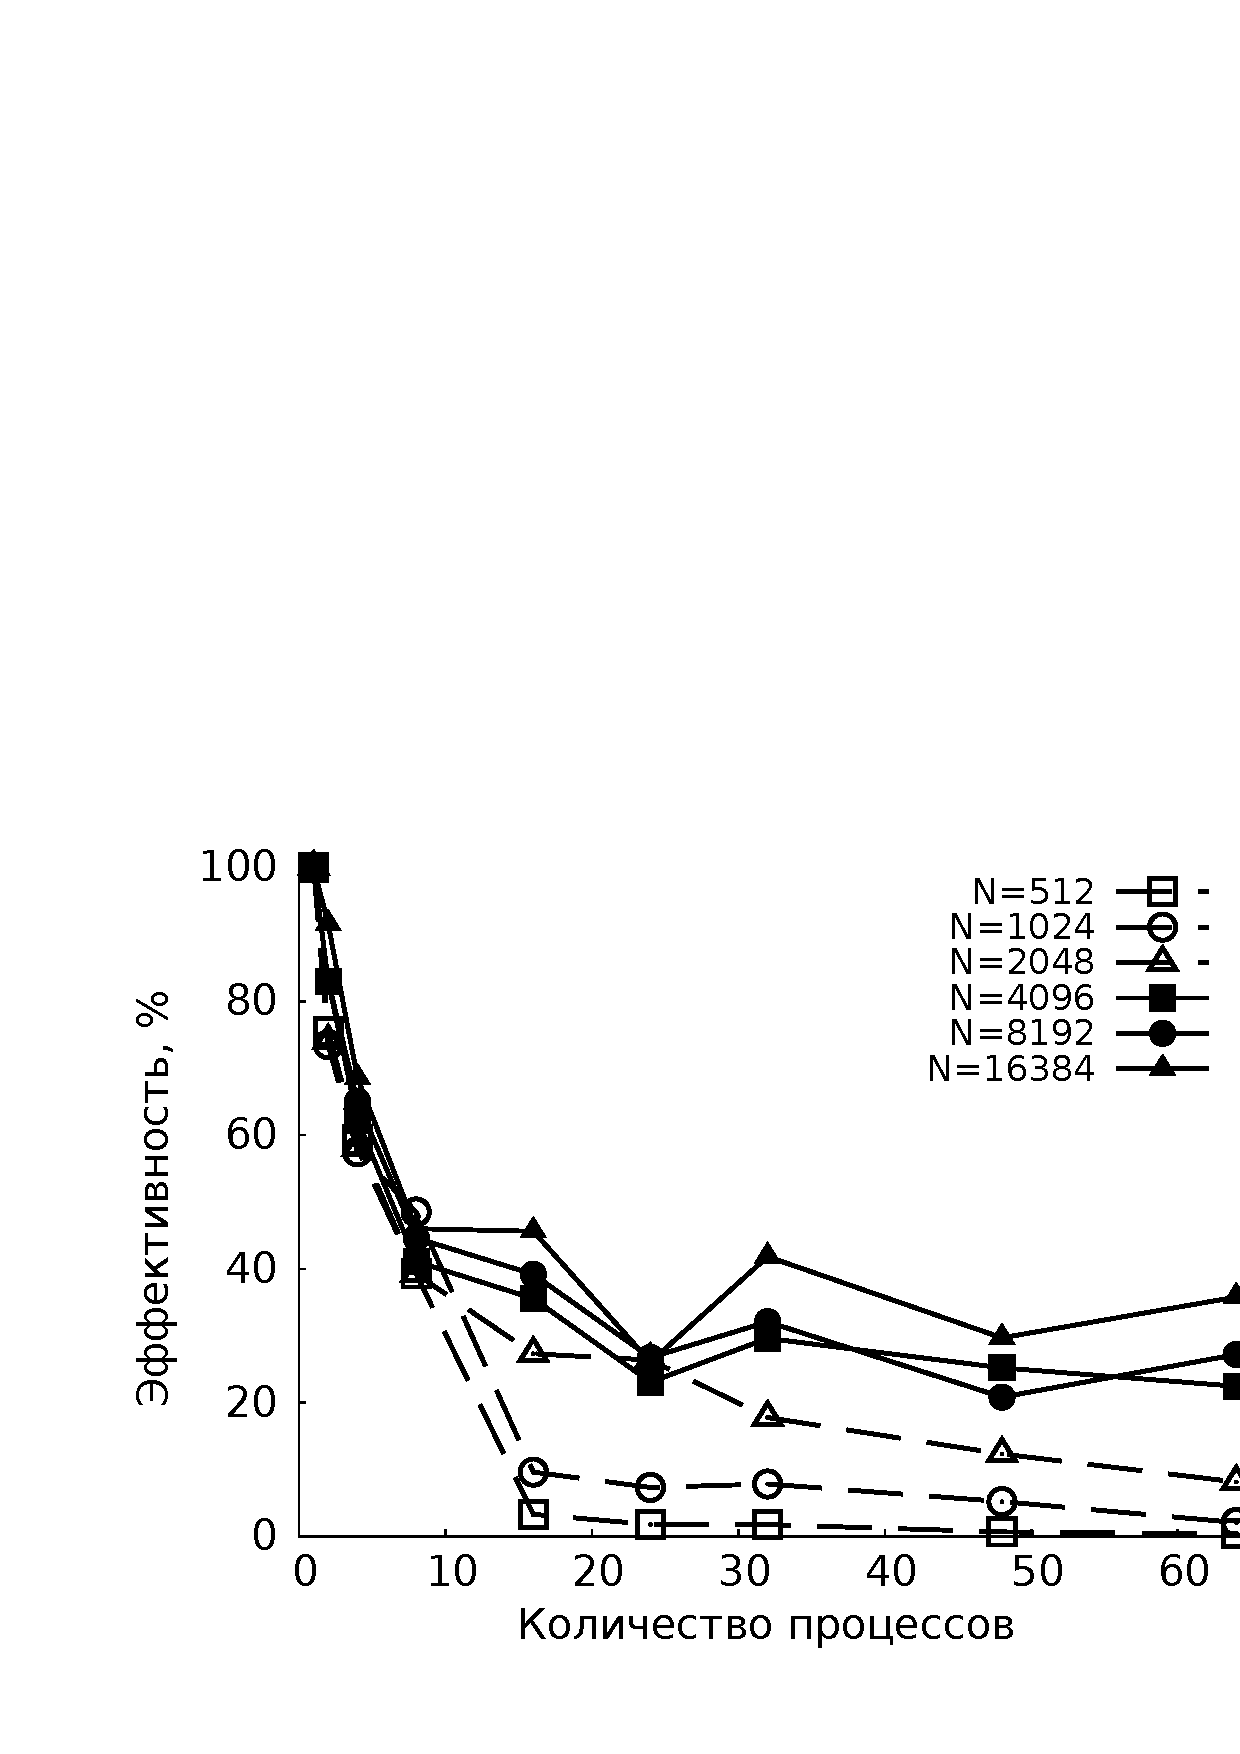
\includegraphics[width=0.95\linewidth]{\graphsdir/Skif/FFTW_efficiency_withsave_all.png}} \\
                \caption{Эффективность Фурье-алгоритма в зависимости от количества процессов для разных размеров матриц. Сохранение данных в файл производилось на каждом десятом шаге.}
                \label{gr:EfficiencyFourierSave}
			\end{minipage}
		\end{center}
	\end{figure}

Были проведены замеры времени для лучшего набора опций (отсутствие буфера, FFTW\_TRANSPOSED\_ORDER, FFTW\_ESTIMATE).
Замеры проводились без сохранения матрицы в файл и с параллельной записью матрицы в файл на каждом десятом шаге.
Рассчитанные по полученным данным ускорения и эффективности программ представлены на рис. \ref{gr:SpeedupFourierNosave}--\ref{gr:EfficiencyFourierSave}.
Видно, что для размера матрицы поля, не превосходящего $2048\times2048$, использование более 8 процессов нецелесообразно, поскольку не дает прироста скорости.
Эффективность реализации резко падает для размеров матрицы поля $512\times512$ и $1024\times1024$. 
Для больших матриц эффективность остается значительной: около 50\% для случая без сохранения данных и около 30\% для случая с сохранением.
    \begin{figure}[h!]
        \begin{center}
            \begin{minipage}{0.45\linewidth}
                \center{
                    \includegraphics[width=0.95\linewidth]{\graphsdir/Skif/Sweep_acceleration_nosave_all.png}
                } 
                \caption{Ускорение параллельного алгоритма с неявной схемой. СКИФ МГУ. Сохранение данных в файл не производилось.}
                \label{gr:SweepSpeedupSkifNosave}
			\end{minipage}
			\hfill
			\begin{minipage}{0.45\linewidth}
                \center{
                    \includegraphics[width=0.95\linewidth]{\graphsdir/Skif/Sweep_acceleration_withsave_all.png}
                }
                \caption{Ускорение параллельного алгоритма с неявной схемой. СКИФ МГУ. Сохранение данных в файл производилось на каждом десятом шаге.}
                \label{gr:SweepSpeedupSkifSave}
			\end{minipage}
		\end{center}
	\end{figure}

    \begin{figure}[h!]
        \begin{center}
            \begin{minipage}{0.45\linewidth}
                \center{
                    \includegraphics[width=0.95\linewidth]{\graphsdir/Skif/Sweep_efficiency_nosave_all.png}
                }
                \caption{Эффективность параллельного алгоритма с неявной схемой. СКИФ МГУ. Сохранение данных в файл не производилось.}
                \label{gr:SweepEfficiencySkifNosave}
			\end{minipage}
			\hfill
			\begin{minipage}{0.45\linewidth}
				\center{
                    \includegraphics[width=0.95\linewidth]{\graphsdir/Skif/Sweep_efficiency_withsave_all.png}
                }
                \caption{Эффективность параллельного алгоритма с неявной схемой. СКИФ МГУ. Сохранение данных в файл производилось на каждом десятом шаге.}
                \label{gr:SweepEfficiencySkifSave}
			\end{minipage}
		\end{center}
	\end{figure}

Для алгоритма, использующего неявную схему, проводились замеры времени работы на кластерах СКИФ МГУ <<Чебышёв>> и IBM BlueGene/P.

Результаты замеров времени на СКИФе представлены на рис. \ref{gr:SweepSpeedupSkifNosave}--\ref{gr:SweepEfficiencySkifSave}.
Большие размеры матрицы не позволяли произвести расчет с использованием одного процесса, поэтому нормировка производилась на время работы программы на 4 процессах.

Видно, что при сохранении результатов в ходе работы программы, для матриц размером 512 и 1024 при увеличении числа процессов от 8 до 32 ускорение падает.

Эффективность работы программы при сохранении результатов в ходе работы уменьшается, относительно эффективности работы программы не сохраняющей результаты расчетов в файлы. Увеличение числа процессов эффективно при размере матрицы более 1024, если происходит сохранение результатов.
	\begin{figure}[h!]
		\begin{center}
			\begin{minipage}{0.45\linewidth}
				\center{
                    \includegraphics[width=0.95\linewidth]{\graphsdir/Bluegene/Sweep_acceleration_nosave_all.png}
                }
                \caption{Ускорение параллельного алгоритма с неявной схемой. BlueGene/P. Сохранение данных в файл не производилось.}
                \label{gr:SweepSpeedupBluegeneNosave}
			\end{minipage}
			\hfill
			\begin{minipage}{0.45\linewidth}
                \center{
                    \includegraphics[width=0.95\linewidth]{\graphsdir/Bluegene/Sweep_acceleration_withsave_all.png}
                }
                \caption{Ускорение параллельного алгоритма с неявной схемой. BlueGene/P. Сохранение данных в файл производилось на каждом десятом шаге.}
                \label{gr:SweepSpeedupBluegeneSave}
			\end{minipage}
		\end{center}
	\end{figure}
    \begin{figure}[h!]
        \begin{center}
            \begin{minipage}{0.45\linewidth}
                \center{
                    \includegraphics[width=0.95\linewidth]{\graphsdir/Bluegene/Sweep_efficiency_nosave_all.png}
                }
                \caption{Эффективность параллельного алгоритма с неявной схемой. BlueGene/P. Сохранение данных в файл не производилось.}
                \label{gr:SweepEfficiencyBluegeneNosave}
            \end{minipage}
            \hfill
            \begin{minipage}{0.45\linewidth}
                \center{
                    \includegraphics[width=0.95\linewidth]{\graphsdir/Bluegene/Sweep_efficiency_withsave_all.png}
                }
                \caption{Эффективность параллельного алгоритма с неявной схемой. BlueGene/P. Сохранение данных в файл производилось на каждом десятом шаге.}
                \label{gr:SweepEfficiencyBluegeneSave}
            \end{minipage}
        \end{center}
    \end{figure}
    
Результаты замеров времени работы алгоритма с использованием неявной схемы на кластере IBM Bluegene/P приведены на рис. \ref{gr:SweepSpeedupBluegeneNosave}--\ref{gr:SweepEfficiencyBluegeneSave}.

Большие размеры матрицы не позволяли произвести расчет с использованием одного процесса, поэтому нормировка производилась на время работы программы на 8 процессах. Видно стабильное линейное увеличение ускорения работы программы при увеличении числа процессоров уже для сравнительно небольших матриц.
Эффективность реализации близка к единице.
Таким образом, при работе на IBM Bluegene/P, увеличение числа процессов, на которых запускается программа,
эффективно. Однако, время выполнения шага интегрирования на IBM Bluegene/P существенно больше, чем на СКИФе, что связано с существенно более слабыми процессорами. 
